\documentclass[dvipdfmx]{jsarticle}


\usepackage{tcolorbox}
\usepackage{color}
\usepackage{listings, plistings}

%% ノート/latexメモ
%% http://pepper.is.sci.toho-u.ac.jp/pepper/index.php?%A5%CE%A1%BC%A5%C8%2Flatex%A5%E1%A5%E2

% Java
\lstset{% 
  frame=single,
  backgroundcolor={\color[gray]{.9}},
  stringstyle={\ttfamily \color[rgb]{0,0,1}},
  commentstyle={\itshape \color[cmyk]{1,0,1,0}},
  identifierstyle={\ttfamily}, 
  keywordstyle={\ttfamily \color[cmyk]{0,1,0,0}},
  basicstyle={\ttfamily},
  breaklines=true,
  xleftmargin=0zw,
  xrightmargin=0zw,
  framerule=.2pt,
  columns=[l]{fullflexible},
  numbers=left,
  stepnumber=1,
  numberstyle={\scriptsize},
  numbersep=1em,
  language={Java},
  lineskip=-0.5zw,
  morecomment={[s][{\color[cmyk]{1,0,0,0}}]{/**}{*/}},
  keepspaces=true,         % 空白の連続をそのままで
  showstringspaces=false,  % 空白字をOFF
}
%\usepackage[dvipdfmx]{graphicx}
\usepackage{url}
\usepackage[dvipdfmx]{hyperref}
\usepackage{amsmath, amssymb}
\usepackage{itembkbx}
\usepackage{eclbkbox}	% required for `\breakbox' (yatex added)
\usepackage{enumerate}
\fboxrule=0.5pt
\parindent=1em
\begin{document}

%\anaumeと入力すると穴埋め解答欄が作れるようにしてる。\anaumesmallで小さめの穴埋めになる。
\newcounter{mycounter} % カウンターを作る
\setcounter{mycounter}{0} % カウンターを初期化
\newcommand{\anaume}[1][]{\refstepcounter{mycounter}{#1}{\boxed{\phantom{aa}\themycounter \phantom{aa}}}} %穴埋め問題の空欄作ってる。
\newcommand{\anaumesmall}[1][]{\refstepcounter{mycounter}{#1}{\boxed{\tiny{\phantom{a}\themycounter \phantom{a}}}}}%小さい版作ってる。色々改造できる。

%% 修正時刻: Tue May  5 10:19:29 2020


\section{Webサーバーを動かす}

\subsection{作業フォルダでHTMLファイルを作成}

適当なフォルダに作業フォルダを作る。

ここでは作業フォルダを \textsf{test} とする。

その \textsf{test} の中に、index.html を作成する。
内容は以下。

\begin{lstlisting}[caption=index.html]
 <!doctype html>
 <html lang="ja">
   <head>
     <meta charset="utf-8">
     <title>TEST</title>
   </head>
   <body>
     <h1>TEST</h1>
   </body>
 </html>
\end{lstlisting}


\subsection{簡易Webサーバーを起動}

\textsf{test}フォルダでコマンドプロンプトを起動する。

以下のコマンドを実行する。

\begin{tcolorbox}
 $>$ \textsf{php -S localhost:8888}
\end{tcolorbox}

すると、以下のような文字列が表示され、Webサーバーが起動したことがわかる。

\vspace{3mm}
\begin{tabular}{|l|} \hline
\verb![Sat Aug ...(略)...] PHP 8.0.9 Development Server (http://localhost:8888) started! \\ \hline
\end{tabular}
\vspace{3mm}


ブラウザで \textsf{http://localhost:8888/} にアクセスしてみる。

\vspace{3mm}
\begin{tabular}{|c|} \hline
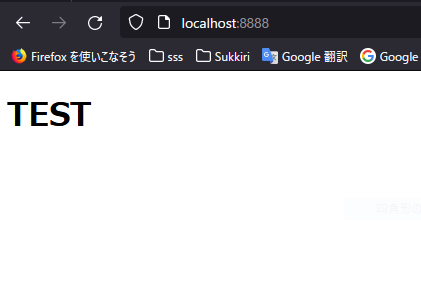
\includegraphics{../img/21-web-test.png} \\ \hline
\end{tabular}
\vspace{3mm}


先ほど作成した \textsf{index.html} が表示される。

\section{TelnetでWebサーバーと通信する}

\subsection{Telnetとは}

\textsf{Telnet} とは、``ネットワークを経由して別のコンピュータに接続し、そのコンピュータを操作する''
ためのプロトコルである。

そのプロトコルを使った通信のためのツールが telnet (同じ名前)。

昔からあるツールだけど、
現在でも、いろいろなサーバを管理するのに、そのサーバに接続するためのツールとして使われている。

ここでいう''接続''とは、ネットワーク越しに離れたコンピュータにコマンドを送ったりすること。
つまり、``通信する''ということ。

``telnet.exe''というプログラムが Windowsにはあるけれど、キョーレツ使いにくいので、\textsf{TeraTerm}を使う。


\subsection{TeraTermの設定}

まず、使うための準備が必要である。

TeraTermがインストールされたフォルダ \textsf{C:\yen Program Files (x86)\yen teraterm} を開ける。

その中に、\textsf{TERATERM.INI} というファイルがあるので、念のため、バックアップのためのコピーを
作っておいて (``TERATERM.INI\_org''というファイル名にしておく)、\textsf{TERATERM.INI} を
\textsf{TeraPad} で開く。

\begin{tcolorbox}
 TCPLocalEcho=off \\
 TCPCRSend=
\end{tcolorbox}

と書かれた箇所を検索して探し出し、(たぶん 680行目くらい)、以下のように修正する。

\begin{tcolorbox}
 TCPLocalEcho=\textsf{on} \\
 TCPCRSend=\textsf{CRLF}
\end{tcolorbox}

以下のように修正する。

\vspace{3mm}
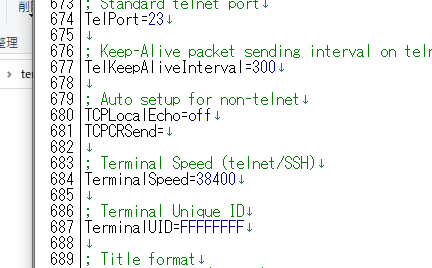
\includegraphics[width=10cm]{../img/22-teraterm-ini.png}
\vspace{3mm}

\vspace{3mm}
\hspace{5cm}

\includegraphics[width=6mm]{../img/arrow-down-s.png}
\vspace{3mm}

\vspace{3mm}
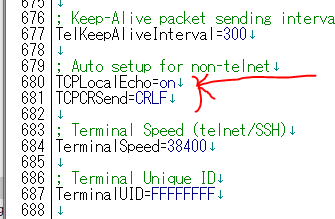
\includegraphics[width=10cm]{../img/23-teraterm-after.png}
\vspace{3mm}

\vspace{10mm}
次に TeraTerm を起動する。

起動したら、``キャンセル'' として、以下の設定をおこなう。

\newpage
 ``設定'' ------ ``TCP/IP'' と選択する。

``\textgt{自動的にウィンドウを閉じる}'' のチェックをはずす。

\vspace{3mm}
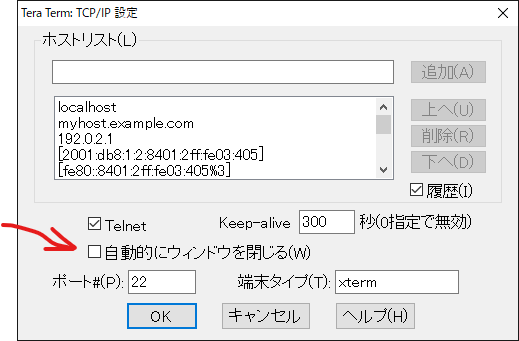
\includegraphics{../img/24-auto-close.png}
\vspace{3mm}

``設定'' ------ ''設定の保存'' を選択。``TERATERM.INI''に上書き保存する。

TeraTermを終了する。









\end{document}

%% 修正時刻: Sat May  2 15:10:04 2020



%% 修正時刻: Sat Aug 21 19:07:57 2021
% \verb!""